\documentclass{article}%
\usepackage[T1]{fontenc}%
\usepackage[utf8]{inputenc}%
\usepackage{lmodern}%
\usepackage{textcomp}%
\usepackage{lastpage}%
\usepackage[head=40pt,margin=0.5in,bottom=0.6in]{geometry}%
\usepackage{graphicx}%
%
\title{\textbf{Denuncian que el general Baduel tiene 10 semanas aislado}}%
\author{El Nacional Web}%
\date{12/10/2018}%
%
\begin{document}%
\normalsize%
\maketitle%
\textbf{URL: }%
http://www.el{-}nacional.com/noticias/presos{-}politicos/denuncian{-}que{-}general{-}baduel{-}tiene{-}semanas{-}aislado\_255472\newline%
%
\textbf{Periodico: }%
EN, %
ID: %
255472, %
Seccion: %
Presos políticos\newline%
%
\textbf{Palabras Claves: }%
Política, Presos políticos, Sebin, Gobierno\newline%
%
\textbf{Derecho: }%
1.2, %
Otros Derechos: %
1.3, %
Sub Derechos: %
1.2.2, 1.3.2.1\newline%
%
\textbf{EP: }%
NO\newline%
\newline%
%
\textbf{\textit{Andreina Baduel calificó la medida como un acto injustificado~}}%
\newline%
\newline%
%
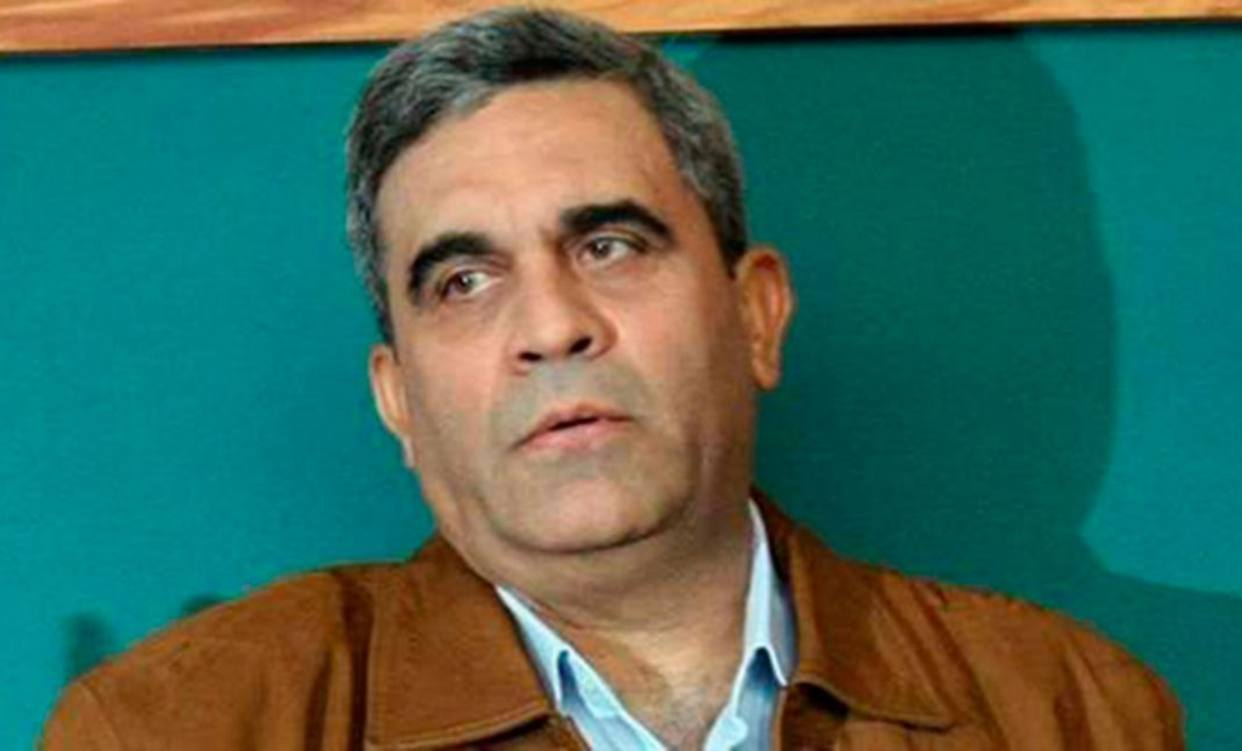
\includegraphics[width=300px]{77.jpg}%
\newline%
%
La hija del general Raúl Baduel, Andreina Baduel, denunció que~ su padre cumplió 10 semanas aislado en la sede del Servicio Bolivariano de Inteligencia Nacional (Sebin) en Plaza Venezuela.%
\newline%
%
Calificó la medida como un acto injustificado y señaló que se trata del segundo aislamiento al que el general Baudel es sometido durante 2018.%
\newline%
%
“La tumba es uno de los centros de tortura del régimen para quienes piensan distinto”, aseguró.%
\newline%
%
Andreina Baudel explicó que solo pudieron ver al general durante junio y julio, y acotó que durante el proceso han sido escoltados por funcionarios del lugar y grabados por un camarógrafo.%
\newline%
%
\end{document}